\documentclass[12pt]{beamer}
\usepackage[utf8]{inputenc}
\usepackage[T1]{fontenc}
\usepackage[portuguese]{babel}
\usepackage{graphicx}
\usepackage{color}
\usepackage{slidesdef}

\title{Git - Trabalhando com repositórios}
\author{Laboratório de Pesquisa Operacional e Otimização \\
  Abel Siqueira \\
  Raniere Silva
}

\date{ 27 de Setembro de 2014 }

\newcommand{\cmd}[1]{
\begin{flushleft}
{\color{yellow} \tt \$ #1 }\\
\end{flushleft}
}

\newcommand{\cmdinline}[1]{
{\color{yellow} \tt #1} }

\newcommand{\cmmt}[1]{
{\color{magenta} \tt \# #1} }

\newcommand{\bashgt}{ \textgreater\ }
\newcommand{\ddash}{-{}-}

\begin{document}

\myframe{
  \maketitle
}

\tikzstyle{local}=[draw, rectangle]
\tikzstyle{remoto}=[draw, circle]

\myframe{
  \begin{center}
    \begin{tikzpicture}[thick, node distance=3cm, bend angle=20, shorten <=1pt,
      shorten >=1pt, bend right]
      \node[local] (voce)   {Você};
      \onslide<2->{
        \node[remoto] (remote) [above right of=voce] {Remoto};
        \draw[->] (voce) to (remote);
      }
      \onslide<3->{
        \draw[->] (remote) to (voce);
      }
      \onslide<4->{
        \node[local] (note) [below right of=remote] {Notebook};
        \draw[->] (note) to (remote);
        \draw[->] (remote) to (note);
      }
      \onslide<5->{
        \node[remoto] (fork) [above of=remote] {Fork};
        \draw[->] (remote) to (fork);
      }
      \onslide<6->{
        \draw[->] (fork) to (remote);
        \draw[->] (fork) to (voce);
        \draw[->, bend left] (fork) to (note);
      }

    \end{tikzpicture}
  \end{center}
}

\myframe{
  \ctr{Repositórios online}
  \begin{itemize}
    \item \only<1>{GitHub}\only<2>{{\color{red}\bf GitHub (criem conta agora)}}
    \item Bitbucket
    \item Gitorious
  \end{itemize}
}

\myframetop{
  \ctr{Criando o repositório no GitHub}
  \begin{center}
    \only<1>{ 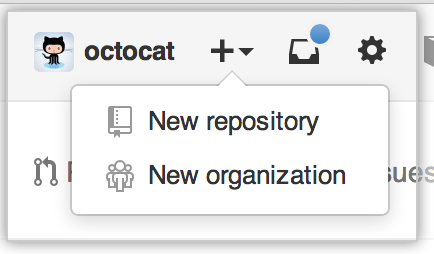
\includegraphics[width=0.8\textwidth]{repo-create.png} }
    \only<2>{ 
\includegraphics[width=0.9\textwidth]{create-repository-name.png} }
    \only<3>{ 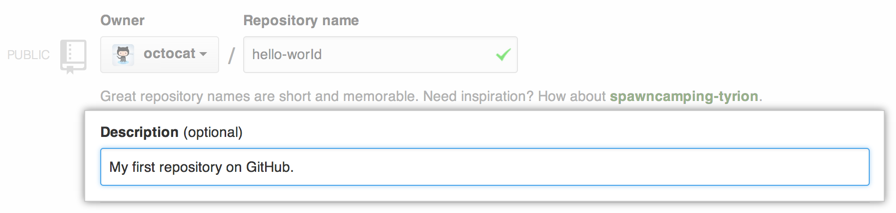
\includegraphics[width=0.9\textwidth]{create-repository-desc.png} }
    \only<4>{ 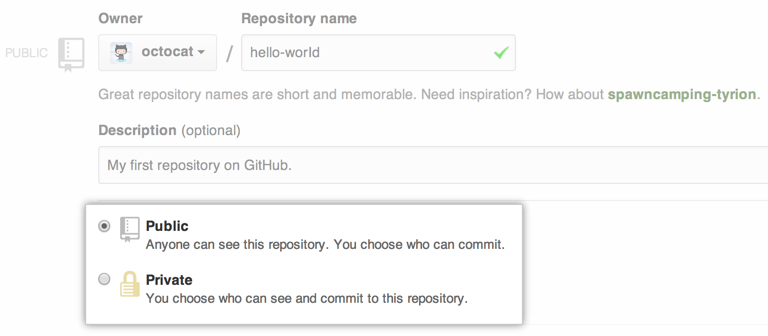
\includegraphics[width=0.9\textwidth]{create-repository-public-private.png} }
    \only<5>{ 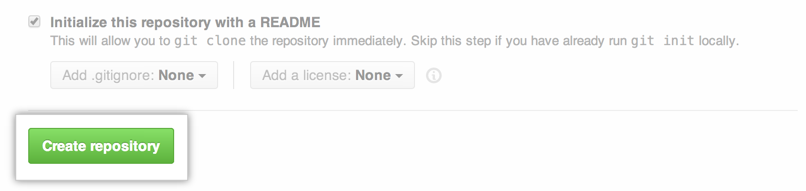
\includegraphics[width=0.9\textwidth]{create-repository-button.png} }
  \end{center}
}

\myframeblack{
  \ctrwhite{No computador}

  \cmd{git remote add origin https://usuario@github.com/usuario/repositorio.git}
  \cmd{git push -u origin master}
}

\myframe{
  \ctr{Trabalhando com algo pronto}
  \ctr{Site: https://github.com/lpoo/git-remoto-exemplo}
  \ctr{Faça um fork}
}

\myframeblack{
  \cmd{git clone https://usuario@github.com/usuario/git-remoto-exemplo}
  \cmd{cd git-remoto-exemplo}
  \cmd{ls}
  \cmd{git log}
  \cmd{cat README.md}
}

\myframe{
  \ctr{Exercício}
  \begin{itemize}
    \item Divide em duplas. Uma pessoa é A e a outra B.
    \item Edite o arquivo {\tt README.md}.
    \item Faça um commit.
  \end{itemize}
}

\myframeblack{
  \cmd{git remote add colega https://github.com/colega/git-remoto-exemplo}
  \cmd{git fetch \ddash all}
  \cmd{git branch -a}
  \cmd{git log \ddash oneline \ddash decorate \ddash all \ddash graph}
}

\myframeblack{
  \ctrwhite{A faz o push}
  \cmd{git push \cmmt{Não precisa de -u origin master}}
  \cmd{git log \ddash oneline \ddash decorate \ddash all \ddash graph}
}

\myframeblack{
  \ctrwhite{B faz fetch, merge, e depois push}
  \cmd{git fetch colegaA}
  \cmd{git log \ddash oneline \ddash decorate \ddash all \ddash graph}
  \cmd{git diff colegaA/master}
  \cmd{git merge colegaA/master \cmmt{Vai dar conflito}}
  \cmd{git status \cmmt{Abre o arquivo e resolve o conflito}}
  \cmd{git commit -am ``mensagem''}
  \cmd{git push}
  \cmd{git log \ddash oneline \ddash decorate \ddash all \ddash graph}
}

\myframeblack{
  \ctrwhite{A faz fetch, merge, e depois push}
  \cmd{git fetch colegaB}
  \cmd{git log \ddash oneline \ddash decorate \ddash all \ddash graph}
  \cmd{git diff colegaB/master}
  \cmd{git merge colegaB/master}
  \cmd{git push}
  \cmd{git log \ddash oneline \ddash decorate \ddash all \ddash graph}
}

\myframe{
  \begin{center}
    \ctr{Workflow}
    \begin{tikzpicture}[thick, node distance=3cm, shorten <=1pt, shorten >=1pt]
      \node[local] (localA) {A local};
      \onslide<2->{
        \node[remoto] (remoteA) [above of=localA] {A remoto};
        \draw[->] (localA) to (remoteA);
      }
      \onslide<3->{
        \node[local] (localB) [right of=localA] {B local};
        \draw[->] (remoteA) to (localB);
      }
      \onslide<4->{
        \node[remoto] (remoteB) [above of=localB] {B remoto};
        \draw[->] (localB) to (remoteB);
      }
      \onslide<5->{
        \draw[->] (remoteB) to (localA);
      }

    \end{tikzpicture}
  \end{center}
}

\myframe{
  \begin{center}
    \ctr{Workflow}
    \begin{tikzpicture}[thick, node distance=3cm, shorten <=1pt, shorten >=1pt]
      \node[local] (localB) {B local};
      \node[remoto] (remote) [above of=localB] {Remoto};
      \node[local] (localA) [left of=localB] {A local};
      \node[local] (localC) [right of=localB] {C local};
      \draw[<->] (remote) to (localA);
      \draw[<->] (remote) to (localB);
      \draw[<->] (remote) to (localC);
    \end{tikzpicture}
  \end{center}
}

\myframecolor{green!50!black}{
  \ctrcolor{green}{\Large Faça}
  \ctrwhite{Suba os commits para o remoto}
  \ctrwhite{Escolha um workflow}
  \ctrwhite{Use branches para separar seu trabalho}
}

\myframecolor{red!50!black}{
  \ctrcolor{red}{\Large Não Faça}
  \ctrwhite{Não desfaça/refaça commits que forem subidos}
  \ctrwhite{Não renomeie seu repositório}
  \ctrwhite{Se for fazer uma cópia de um trabalho, faça um fork}
}

\myframe{
  \ctr{Outras ferramenta}
  \begin{itemize}
    \item GitHub pages
    \item Travis-CI
    \item Read the Docs (documentação em Sphinx)
    \item Gitter
  \end{itemize}
}

\myframecolor{gray!50!black}{
  \ctrwhite{Sumário}
  \cmd{git remote add <name> <url>}
  \cmd{git push}
  \cmd{git fetch}
  \cmd{git merge}
}

\myframe{
  \ctr{Materiais e Referências}
  \begin{itemize}
    \item \url{git-scm.com}
    \item \url{help.github.com}
    \item \url{http://www.xmind.net/m/RGZm/}
    \item google git cheat sheet
  \end{itemize}
}

\myframe{
  \ctr{\Huge Fim}
}

\end{document}
